\subchapter{Bootloader - TF-A and U-Boot}{Objectives: Set up serial
  communication, understand the AM62x Bootprocess, compile and install the
  U-Boot bootloader, use basic U-Boot commands, set up TFTP communication
  with the development workstation.}

As the bootloader is the first piece of software executed by a
hardware platform, the installation procedure of the bootloader is
very specific to the hardware platform. There are usually two cases:

\begin{itemize}

\item The processor offers nothing to ease the installation of the
  bootloader, in which case the JTAG has to be used to initialize
  flash storage and write the bootloader code to flash. Detailed
  knowledge of the hardware is of course required to perform these
  operations.

\item The processor offers a monitor, implemented in ROM, and through
  which access to the memories is made easier.

\end{itemize}

The AM625 SoC on the BeaglePlay falls into the second category. The monitor
integrated in the ROM reads the SD card or any other interface to search for
a valid bootloader. If this first interface cannot provide a valid bootloader,
the ROM can search somewhere else or will operate in a fallback mode, that will allow
to use an external tool to reflash some executable through USB.

On BeaglePlay board these two options can be chosen with the \code{USR}
key, available on the side of the board\footnote{If you want to know more about
the boot procedure of the AM62x SoC, please refer to AM62x datasheet
(\url{https://www.ti.com/lit/pdf/spruiv7})}.

\begin{center}
    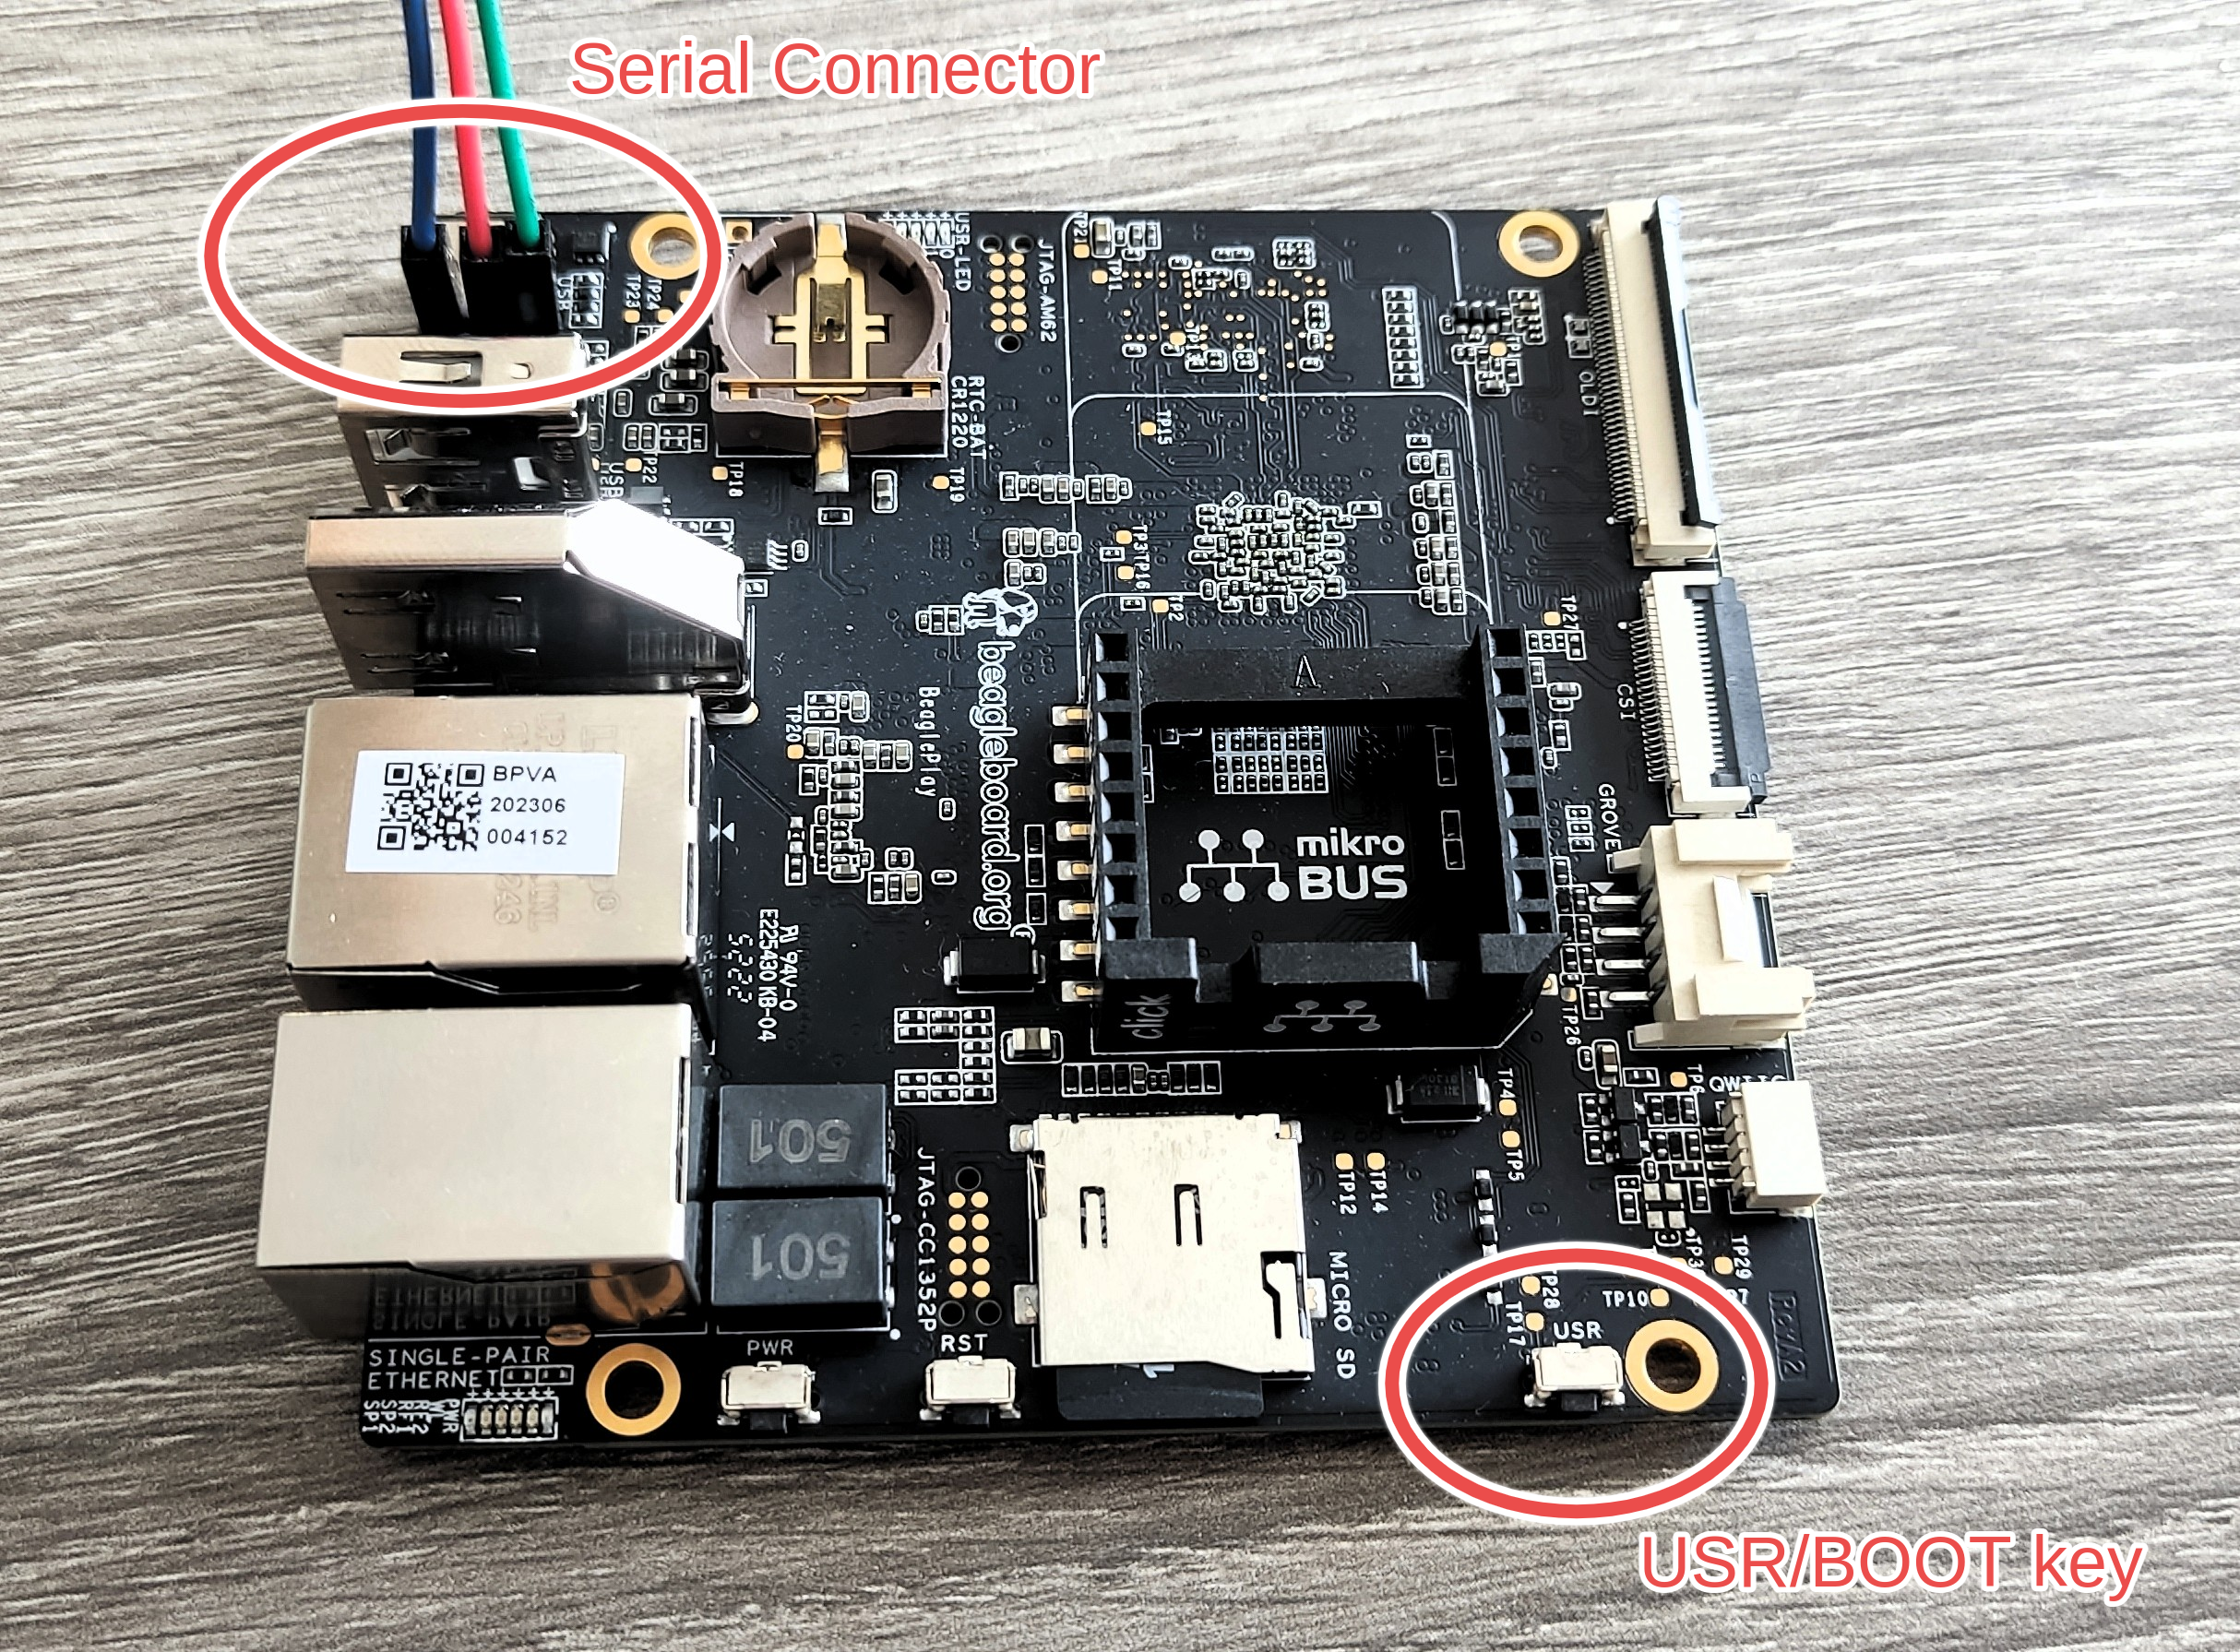
\includegraphics[width=8cm]{labs/sysdev-u-boot-beagleplay/Beagleplay_USRkey_UART.png}
\end{center}

If the \code{USR} key is released, then the SoC will try to find a
bootloader into eMMC memory.
If the \code{USR} key is pressed, then it will try to find a bootloader
on the microSD.

{\bf Warning}: In this tutorial we will boot exclusively on the SD card. Therefore
we will \textbf{ALWAYS} press the \code{USR} key during startup!

Go to the \code{$HOME/__SESSION_NAME__-labs/bootloader} directory.

\section{Setting up serial communication with the board}
The BeaglePlay serial connector is exported on 3 pins near USB-A
and USB-C ports. Using your special USB to Serial adapter provided
by your instructor, connect the ground wire (blue) to the \code{G} pin, the
\code{TX} wire (red) to the \code{RX} pin and finally the \code{RX} wire (green)
to the \code{TX} pin.\footnote{See
\url{https://www.olimex.com/Products/Components/Cables/USB-Serial-Cable/USB-Serial-Cable-F/}
for details about the USB to Serial adapter that we are using.}.

You always should make sure that you connect the \code{TX} pin of the cable
to the \code{RX} pin of the board, and vice versa, whatever the board and
cables that you use. You can look at the picture a few lines above.

Once the USB to Serial connector is plugged in, a new serial port
should appear: \code{/dev/ttyUSB0}.

You can also see this device appear by looking at the output of
\code{sudo dmesg}.

To communicate with the board through the serial port, install a
serial communication program, such as \code{picocom}:

\bashcmd{$ sudo apt install picocom}

If you run {\tt ls -l \hosttty}, you can also see that only
\code{root} and users belonging to the \code{dialout} group have
read and write access to the serial console. Therefore, you need
to add your user to the \code{dialout} group:

\bashcmd{$ sudo adduser $USER dialout}

{\bf Important}: for the group change to be effective, you have to
reboot your computer (at least on Ubuntu 22.04) and log in again.
A workaround is to run \code{newgrp dialout}, but it is not global.
You have to run it in each terminal.

Run {\tt picocom -b 115200 \hosttty}, to start serial
communication on {\tt \hosttty}, with a baudrate of 115200.
If you wish to exit \code{picocom}, press \code{[Ctrl][a]} followed by
\code{[Ctrl][x]}.

There should be nothing on the serial line so far, as the board is not
powered up yet.

It is now time to power up your board by plugging in the type C USB
cable supplied by your instructor to your PC.

See what messages you get on the serial line. You should see U-Boot
start on the serial line, if there was a valid U-Boot and SPL on the
board's eMMC.

\section{Understanding AM62x boot process}

The AM62x SoC Boot Process is quite complex, involving both numerous
hardware and software components.
Let's describe the SoC architecture a little bit more.

The AM62x SoC is organized around 3 hardware domains.

First, we have the MAIN domain, which contains the majority of peripherals and
where the 4 Cortex-A53 processors are located. These processors will be used to
run our linux kernel or our future userspace applications.

Next, we have the MCU domain. The principal advantage of this domain is the
fact that it is isolated from the rest of the SoC and, therefore, provides
safety use cases. This domain is controlled by a Cortex-M4F processor.

Finally, we have the WKUP domain which, as its name suggests, is used during
deepsleep mode and is controlled by a Cortex-R5F processor.

\textbf{Note :} The Cortex-R5F and the Cortex-M4F are 32 bit processors
(in opposition to 64 bit Cortex-A53 processors) and will therefore need
a 32 bit toolchain.

The purpose of the AM62x SoC boot process is to initialize all the required
peripherals and processors in different steps we are about to describe :

The datasheet describes a software component called TIFS, which stands for
TI Foundational Security and is responsible for the Secure
Boot and Power/Ressource Management requests made by the CPUs inside the SoC.

As Master of the boot process, the TIFS, which is running on the M4F processor,
will first initiate the R5 Processor and requests the R5 to load a
complementary firmware to TIFS core.
Once this done the R5 will run a U-Boot SPL in order to configure DDR and
the R5 firmware. Finally it will request the TIFS to start the first A53 CPU.

Once the A53 is started, it will load TF-A within the secure world.
After this, the A53 will switch to normal world and load U-Boot SPL which
will then load the complete U-Boot image.

The Following Process Flow can be viewed at the following address :
\url{https://u-boot.readthedocs.io/en/latest/board/ti/am62x_sk.html}

\section{Get and install the 32 bit toolchain}

As the AM62x is using 32 bit processors we will need a specific toolchain
to perform cross-compilation of 32 bit firmware.
Although we could use Crosstool-ng to compile this 32 bit toolchain, we will use
a precompiled one in order to save compilation time.
To do so, we will get this toolchain from the official ARM website\footnote{You can download precompiled ARM toolchains for other
target architecture on the following link \url{https://developer.arm.com/downloads/-/arm-gnu-toolchain-downloads/}}.

Let's download and untar it:

\begin{bashinput}
      $ wget -O /tmp/arm-gnu-toolchain-12.2.rel1-x86_64-arm-none-eabi.tar.xz https://developer.arm.com/-/media/Files/downloads/gnu/12.2.rel1/binrel/arm-gnu-toolchain-12.2.rel1-x86_64-arm-none-eabi.tar.xz
      $ tar vxJf /tmp/arm-gnu-toolchain-12.2.rel1-x86_64-arm-none-eabi.tar.xz -C $HOME/x-tools
\end{bashinput}

Doesn't forget to add \code{$HOME/x-tools/arm-gnu-toolchain-12.2.rel1-x86_64-arm-none-eabi/bin/}
to your \code{PATH} environment variable.

Now our 32 bit toolchain is installed into \code{$HOME/x-tools} directory !

\section{Configure U-Boot for R5 Processor}

Because the BeaglePlay board is not yet supported by the mainline U-Boot
source, we will use the forked repository of the BeagleBoard vendor.

\begin{bashinput}
$ git clone https://git.beagleboard.org/beagleplay/u-boot.git
$ cd u-boot/
$ git checkout f036fb
\end{bashinput}

To share more easily U-Boot images across builds, let's create a build directory.

\begin{bashinput}
$ mkdir -p ../build_uboot/r5
\end{bashinput}

Get an understanding of U-Boot's configuration and compilation steps
by reading the \code{README} file, and specifically the {\em Building
the Software} section.

Basically, you need to:

\begin{enumerate}

\item Specify the cross-compiler prefix
(the part before \code{gcc} in the cross-compiler executable name):
\bashcmd{$ export CROSS_COMPILE=arm-none-eabi-}
and the architecture type (we are building for the R5, 32 bit Proc):
\bashcmd{$ export ARCH=arm}

\item Run \inlinebash{$ ls configs/ | grep am62x} to see all predefined
      configurations. The one that supports our board for the R5 processor is
      \code{am62x_evm_r5_defconfig}
\item I our case we need to specify the output directory we've
      created a few lines above by adding the following
      flag \code{O=../build_uboot/r5/}

      Now, run \inlinebash{$ make am62x_evm_r5_defconfig O=../build_uboot/r5/}.

\item Now that you have a valid initial configuration, you can now run \\
  \inlinebash{$ make menuconfig O=../build_uboot/r5/} to further edit your bootloader features.
  \begin{itemize}
    \item In the \code{Environment} submenu, we will configure U-Boot so
    that it stores its environment inside a file called \code{uboot.env}
    in an ext4 filesystem:
    \begin{itemize}
      \item Enable \code{Environment is in a EXT4 filesystem}. Disable all other
          options for environment storage (e.g. MMC, SPI, UBI)
      \item \code{Name of the block device for the environment}: \code{mmc}
      \item \code{Device and partition for where to store the environment in
          EXT4}: \code{1:2}
      \item \code{Name of the EXT4 file to use for the environment}: \code{/uboot.env}
    \end{itemize}

  \item In \code{SPL/TPL} $\rightarrow$ Enable \code{Support EXT filesystems}
  \item In \code{Boot Options} $\rightarrow$ \code{Enable a default value for bootcmd}
        and change the \code{bootcmd value} to : \code{echo 'No bootcmd yet'}.
        That way, U-Boot will not try to load automatically a kernel image and just show
        'No bootcmd yet'.
  \end{itemize}

\item Install the following packages which should be needed to compile U-Boot for
  your board:

  \begin{bashinput}
  $ sudo apt install libssl-dev device-tree-compiler swig \
          python3-distutils python3-dev python3-setuptools
  \end{bashinput}

\item Finally, run \bashcmd{make DEVICE_TREE=k3-am625-r5-beagleplay O=../build_uboot/r5/}
  which will build U-Boot
  \footnote{You can speed up the
  compiling by using the \code{-jX} option with \code{make}, where X
  is the number of parallel jobs used for compiling. Twice the
  number of CPU cores is a good value.}.
  The \code{DEVICE_TREE} variable specifies the specific
  Device Tree that describes our hardware board.
  Because we are using an out-of-tree version of U-Boot, the \code{_defconfig}
  file already configures the device tree correctly, and pass the
  \code{DEVICE_TREE} variable is therefore not mandatory.
  That been said, you just could have run \code{make}.
\end{enumerate}

If you go into \inlinebash{../build_uboot/r5/} you can see all the files
generated during the build process. Keep in mind that we will only use the
SPL image of U-Boot for the R5 booting sequence, which is located in the
\code{spl} directory.

\section{Get the TI firmware and create {\tt tiboot3.bin} image}

Now we have the SPL for the R5 processor, the R5 processor is also responsible
for loading the TIFS complementary firmware. So let's get it,

\begin{bashinput}
$ cd $HOME/__SESSION_NAME__-labs/bootloader
$ git clone https://git.ti.com/cgit/processor-firmware/ti-linux-firmware
$ cd ti-linux-firmware
$ git checkout c126d3864b9faf725ff40e620049ab5d56dedc5b
\end{bashinput}

Next, the AM62x requires both SPL and the TIFS firmware to be grouped into a
single image within a X.509 Certificate encaplusation.

To do so, TI provides us a tool called \code{k3-image-gen}, so let's use it !

Get \code{k3-image-gen},
\begin{bashinput}
$ cd ..
$ git clone https://git.ti.com/cgit/k3-image-gen/k3-image-gen
$ cd k3-image-gen/
$ git checkout 150f1956b4bdcba36e7dffc78a4342df602f8d6e
\end{bashinput}

A few parameters have to be passed to the Makefile,
\begin{itemize}
\item The SoC name: \code{SOC=am62x}
\item The path to the \code{u-boot-spl} image:
    \code{SBL=../build_uboot/r5/spl/u-boot-spl.bin}
\item The path to the to TIFS firmware binary image:
    \code{SYSFW_PATH=../ti-linux-firmware/ti-sysfw/ti-fs-firmware-am62x-gp.bin}
\end{itemize}

In a single command we then have:

\begin{bashinput}
$ make SOC=am62x SBL=../build_uboot/r5/spl/u-boot-spl.bin SYSFW_PATH=../ti-linux-firmware/ti-sysfw/ti-fs-firmware-am62x-gp.bin
\end{bashinput}

\section{Get and compile TF-A}
Get the mainline TF-A sources:

\begin{bashinput}
$ cd ..
$ git clone https://github.com/ARM-software/arm-trusted-firmware.git
$ cd arm-trusted-firmware/
$ git checkout v2.9
\end{bashinput}

Several configuration parameters have to be passed to the Makefile:
\begin{itemize}
\item Change the cross-compiler prefix for the aarch64 cross-compiler,
      either using the environment variable:
      \inlinebash{$ export CROSS_COMPILE=aarch64-linux-}, or just by
      adding it to the \code{make} commande line.
\item The architecture has to be selected (aarch64),
      again either using the environment variable: \code{$ export ARCH=aarch64}
      or just by adding it to the \code{make} commande line.
\item The AM62x SoC platform which is the k3 family is selected
      too with \code{PLAT=k3}
\item And we specify the target board we use with \code{TARGET_BOARD=lite}
\end{itemize}

So the resulting make command is:
\begin{bashinput}
    $ make PLAT=k3 TARGET_BOARD=lite
\end{bashinput}


% We are not forced to use OPTEE and in order to simplify the lab
% we will not using it

% \section{Get and compile OPTEE-OS}
% Get the mainline OPTEE-OS sources:

% \begin{bashinput}
% $ cd ..
% $ git clone https://github.com/OP-TEE/optee_os.git
% $ cd optee_os/
% $ git checkout 3.21.0
% \end{bashinput}

% Several configuration parameters have to be passed to the Makefile:
% \begin{itemize}
% \item Specify the 32 bit cross-compiler prefix \code{CROSS_COMPILE=arm-none-eabi-}
% \item Specify the 64 bit cross-compiler prefix \code{CROSS_COMPILE64=aarch64-linux-}
% \item In order to indicates that our SoC supports both 64 and 32 bit builds,
%       we need to set \code{CFG_ARM64_core=y}
% \item The AM62x SoC platform which is the k3 family is selected
%       too with \code{PLATFORM=k3}
% \end{itemize}

% So the resulting make command is:
% \begin{bashinput}
%     $ make PLATFORM=k3 CFG_ARM64_core=y CROSS_COMPILE=arm-none-eabi- CROSS_COMPILE64=aarch64-linux-
% \end{bashinput}

% You may encounter a building issue if you choose to set ARCH env variable
% beacause Optee will try to load some specific makefiles to your architecture.
% In that case you need to remove this variable with:
% \inlinebash{$ export -n ARCH}

\section{Configure U-boot for the A53 Processor}

First of all, like for the R5, we have to create an output directory:
\begin{bashinput}
$ cd $HOME/__SESSION_NAME__-labs/bootloader
$ mkdir build_uboot/a53/
$ cd u-boot/
\end{bashinput}

For setting-up the A53 U-Boot, we will reuse the previous
U-Boot directory. Few configuration changes are however needed:

\begin{enumerate}
\item Change your shell environment variables to match the new
  target architecture,
  \begin{bashinput}
  $ export ARCH=aarch64
  $ export CROSS_COMPILE=aarch64-linux-
  \end{bashinput}
\item Load the \code{__defconfig} corresponding to the \code{am62x}
  for \code{A53} Processor and point to the A53 output directory we just
  created:
  \begin{bashinput}
  $ make am62x_evm_a53_defconfig O=../build_uboot/a53/
  \end{bashinput}
\item Now we have to tune the same parameters as for the R5 in the menuconfig
  with the following command:
  \begin{bashinput}
  $ make menuconfig O=../build_uboot/a53/
  \end{bashinput}
\item Finally, we just have to call the make command and pass some parameters
  to the makefile:

  \begin{itemize}
  \item The path to the Trusted Firmware (TF-A):
    \code{ATF=$HOME/__SESSION_NAME__-labs/bootloader/arm-trusted-firmware/build/k3/lite/release/bl31.bin}
  \item The path to the Device Management Firmware (DM) which is included
    by the \code{ti-linux-firmware} package we downloaded before:
    \code{DM=$HOME/__SESSION_NAME__-labs/bootloader/ti-linux-firmware/ti-dm/am62xx/ipc_echo_testb_mcu1_0_release_strip.xer5f}
  \item As usual, do not forget to specify the output directory:
    \code{O=../build_uboot/a53}
  \end{itemize}

  \begin{bashinput}
  $ make ATF=$HOME/__SESSION_NAME__-labs/bootloader/arm-trusted-firmware/build/k3/lite/release/bl31.bin DM=$HOME/embedded-linux-beagleplay-labs/bootloader/ti-linux-firmware/ti-dm/am62xx/ipc_echo_testb_mcu1_0_release_strip.xer5f O=../build_uboot/a53
  \end{bashinput}
\end{enumerate}

If you go to \inlinebash{$HOME/__SESSION_NAME__-labs/bootloader/build_uboot/a53/}
you can see that 2 of the 3 files we will use in the next part have been created
(\code{tispl.bin} and \code{u-boot.img})

\section{Preparing a bootable micro-SD card}\label{sec:Prepboot}

The TI romcode will look for the needed images in a FAT partition
on the SD card. To be recognized by the romcode, this partition have
to have a special type and a special {\em Bootable} Flag.

Let's prepare an SD card with such a partition.

Plug the SD card your instructor gave you on your workstation. Type
the \code{sudo dmesg} command to see which device is used by your
workstation. In case the device is \code{/dev/mmcblk0}, you will see
something like

\begin{verbatim}
[46939.425299] mmc0: new high speed SDHC card at address 0007
[46939.427947] mmcblk0: mmc0:0007 SD16G 14.5 GiB
\end{verbatim}

The device file name may be different (such as \code{/dev/sdb}
if the card reader is connected to a USB bus (either internally
or using a USB card reader).

In the following instructions, we will assume that your SD card is
seen as \code{/dev/mmcblk0} by your PC workstation.

Type the \code{mount} command to check your currently mounted
partitions. If SD partitions are mounted, unmount them:

\bashcmd{$ sudo umount /dev/mmcblk0p*}

We will erase the existing partition table by simply zero-ing the
first 16 MiB of the SD card:

\bashcmd{$ sudo dd if=/dev/zero of=/dev/mmcblk0 bs=1M count=16}

Now, let's create the 2 partitions
that we need to boot the board and store U-Boot env. Note that we could have stored the
U-Boot environment variables in the same partition as the bootloader images.
But to demonstrate what U-Boot is capable of, we stored the U-Boot env
into a separate partition.

There exist several utilities to partition a disk, here we will
be using \code{cfdisk}, which is a graphical version \code{fdisk} tool.

\bashcmd{$ sudo cfdisk /dev/mmcblk0}


If \code{cfdisk} asks you to \code{Select a label type} choose \code{dos}.
This corresponds to traditional partitions tables that DOS/Windows would 
understand. \code{gpt} partition tables are needed for disks bigger than 2 TB.

In the \code{cfdisk} interface, delete existing partitions, and then create 2
partitions with the following properties:

\begin{itemize}
\item First Partition
\begin{itemize}
  \item Size: \code{128MB} big
  \item Select \code{primary} partition
  \item Type: \code{W95 FAT32 (LBA)}  (\code{c} choice)
  \item Bootable flag enabled
\end{itemize}

\item Second Partition
\begin{itemize}
  \item Size: \code{300MB} big
  \item Select \code{primary} partition
  \item Type: \code{Linux}  (\code{83} choice)
\end{itemize}
\end{itemize}


Press \code{Write} when you are done.

We will create further partitions in a later lab, when we need them.

To make sure that partition definitions are reloaded on your
workstation, remove the SD card and insert it again.

Now create a FAT32 filesystem on the bootable partiton:
\begin{bashinput}
sudo mkfs.vfat -F 32 -n boot /dev/mmcblk0p1
\end{bashinput}

And an EXT4 filesystem on the second partition.

Note that we used the \code{-O ^metadata_csum} option which allows us to create
the filesystem without enabling metadata check-sums, which U-Boot doesn't
seem to support yet.
\begin{bashinput}
sudo mkfs.ext4 -L env -O ^metadata_csum /dev/mmcblk0p2
\end{bashinput}

You can now make your workstation automatically mount this
partition by removing the SD card and plugging it back. It should
now be mounted on \code{/media/$USER/boot}.

Now, copy the \code{tiboot3.bin} image into the SD card,
\code{tiboot3.bin} is located in the
\code{$HOME/__SESSION_NAME__-labs/bootloader/k3-image-gen}
folder and contains the 32 bit binaries.

Next, copy both the \code{tispl.bin} and \code{u-boot.img} files.
This time, the images contains 64 bit binaries, and therefore are contained
in the \code{$HOME/__SESSION_NAME__-labs/bootloader/build_uboot/a53}
folder.

So we have the following commands:
\begin{bashinput}
$ cp $HOME/__SESSION_NAME__-labs/bootloader/k3-image-gen/tiboot3.bin /media/$USER/boot/
$ cp $HOME/__SESSION_NAME__-labs/bootloader/build_uboot/a53/tispl.bin /media/$USER/boot/
$ cp $HOME/__SESSION_NAME__-labs/bootloader/build_uboot/a53/u-boot.img /media/$USER/boot/

\end{bashinput}

\section{Testing U-Boot}

Insert the SD card in the board slot. To boot the board on the external micro-SD
card, you need to hold the \code{USR} button at the right of the
microSD slot (as seen from above), and then power-up the board through
its USB-C connection, or reset it. You can then release the
\code{USR} button.

Here's what you should get on the serial line:

\begin{verbatim}
U-Boot SPL 2021.01-gf036fbdc25 (Jun 15 2023 - 11:06:38 +0200)
SYSFW ABI: 3.1 (firmware rev 0x0009 '9.0.4--v09.00.04 (Kool Koala)')
SPL initial stack usage: 13408 bytes
Trying to boot from MMC2

Loading Environment from EXT4... ** File not found /uboot.env **
spl_load_fit_image: Skip load 'tee': image size is 0!
** Unable to read "/uboot.env" from mmc1:2 **
Starting ATF on ARM64 core...

NOTICE:  BL31: v2.9(release):v2.9.0
NOTICE:  BL31: Built : 13:55:17, Jun 15 2023

U-Boot SPL 2021.01-gf036fbdc25 (Jun 19 2023 - 17:33:12 +0200)
SYSFW ABI: 3.1 (firmware rev 0x0009 '9.0.4--v09.00.04 (Kool Koala)')
Trying to boot from MMC2


U-Boot 2021.01-gf036fbdc25 (Jun 19 2023 - 17:33:12 +0200)

SoC:   AM62X SR1.0 GP
Model: BeagleBoard.org BeaglePlay
Board: BEAGLEPLAY-A0- rev 02
DRAM:  2 GiB
MMC:   mmc@fa10000: 0, mmc@fa00000: 1, mmc@fa20000: 2
Loading Environment from EXT4... ** File not found /uboot.env **

** Unable to read "/uboot.env" from mmc1:2 **
In:    serial@2800000
Out:   serial@2800000
Err:   serial@2800000
Error: Can't set serial# to SSSS
Net:   Could not get PHY for ethernet@8000000port@1: addr 0
am65_cpsw_nuss_port ethernet@8000000port@1: phy_connect() failed
No ethernet found.

Press SPACE to abort autoboot in 2 seconds
=>
\end{verbatim}

The code above shows us the main steps of the boot process.
First we can see that the SPL bootloader as been loaded by the R5.
Next the TF-A (ATF) is loaded and we jump into the normal boot world.
Finally, the 64 bit U-Boot SPL is loaded which load U-Boot itself.

\textbf{Note:} We can see that the R5 U-Boot SPL skips the 'tee'
image. This is because we chose to not use OPTEE in order
to make the lab easier to understand. If you want to add OPTEE please refer
to the U-Boot Documentation
(\url{https://u-boot.readthedocs.io/en/latest/board/ti/am62x_sk.html}).

Make sure that the version and compile date are right. Otherwise, try
again, because this means that you booted on the internal eMMC.

In U-Boot, type the \code{help} command, and explore the few commands
available.

\subsection{Adding a new command to the U-Boot shell}

Check whether the \code{config} command is available. This command
allows to dump the configuration settings U-Boot was compiled from.

If it's not, go back to U-Boot's configuration and enable it.

Re-run the build of U-Boot, and update the bootloader on the SD card
and test that the command is now available and works as expected.

\subsection{Playing with the U-Boot environment}

Display the U-Boot environment using \code{printenv}\footnote{Note that
the environment is already pretty full. This is beacause the selected
U-Boot configuration already include default variables to help us configure
the board}.

Set a new U-Boot variable \code{foo} to a value of your choice, using
\code{setenv}, and verify it has been set. Reset the board, and check
if \code{foo} is still defined: it should not.

Now repeat this process, but before resetting the board, use
\code{saveenv}. After the reset, check the \code{foo} variable is
still defined.

Now reset the environment to its default settings using \code{env
  default -a}, and save these changes using \code{saveenv}.

\section{Setting up networking}

The next step is to configure U-boot and your workstation to let your
board download files, such as the kernel image and Device Tree Binary
(DTB), using the TFTP protocol through a network connection.

With a network cable, connect the Ethernet port of
your board to the one of your computer. If your computer already has a
wired connection to the network, your instructor will provide you with
a USB Ethernet adapter. A new network interface should appear on your
Linux system.

\subsection{Network configuration on the target}

Let's configure networking in U-Boot:

\begin{itemize}
\item \code{ipaddr}: IP address of the board
\item \code{serverip}: IP address of the PC host
\end{itemize}

\begin{ubootinput}
=> setenv ipaddr 192.168.0.100
=> setenv serverip 192.168.0.1
\end{ubootinput}

Of course, make sure that this address belongs to a separate network
segment from the one of the main company network.

To make these settings permanent, save the environment:

\begin{ubootinput}
=> saveenv
\end{ubootinput}

\subsection{Network configuration on the PC host}

To configure your network interface on the workstation side, we need
to know the name of the network interface connected to your board.

Find the name of this interface by typing:
\bashcmd{=> ip a}

The network interface name is likely to be
\code{enxxx}\footnote{Following the {\em Predictable Network Interface
Names} convention:
\url{https://www.freedesktop.org/wiki/Software/systemd/PredictableNetworkInterfaceNames/}}.
If you have a pluggable Ethernet device, it's easy to identify as it's
the one that shows up after pluging in the device.

Then, instead of configuring the host IP address from NetworkManager's
graphical interface, let's do it through its command line interface,
which is so much easier to use:

\bashcmd{$ nmcli con add type ethernet ifname en... ip4 192.168.0.1/24}

\section{Setting up the TFTP server}

Let's install a TFTP server on your development workstation:

\begin{verbatim}
sudo apt install tftpd-hpa
\end{verbatim}

You can then test the TFTP connection. First, put a small text file in
the directory exported through TFTP on your development
workstation. Then, from U-Boot, do:

\begin{ubootinput}
=> tftp %\zimageboardaddr% textfile.txt
\end{ubootinput}

The \code{tftp} command should have downloaded the
\code{textfile.txt} file from your development workstation into
the board's memory at location {\tt \zimageboardaddr}\footnote{
This location is part of the board SDRAM. If you want
to check where this value comes from, you can check the SoC
datasheet at
\url{https://www.ti.com/lit/ug/spruiv7a/spruiv7a.pdf}.
It's a big document (more than 12,000 pages). In this document, look
for \code{Memory Map} and you will find the SoC memory map.
You will see that the address range for the memory controller
({\em DDR16SS0\_SDRAM})
starts at the address we are looking for.
You can also try with other values in the RAM address range.}.

You can verify that the download was successful by dumping the
contents of the memory:

\begin{ubootinput}
=> md %\zimageboardaddr%
\end{ubootinput}

We will see in the next labs how to use U-Boot to download, flash and
boot a kernel.

\section{Optional: Flash the bootloader onto eMMC memory}
If this is too inconvenient for you to hold the \code{USR}
button every time your board boots, you could use U-Boot on the external
micro-SD card to flash the bootloader files onto the onboard eMMC memory.

When the Beagleplay is booting up on eMMC, it will first look at the
\code{boot0} hardware partition\footnote{To know more about hardware partitions
on eMMC, please refer to the following link:
\url{https://www.pengutronix.de/en/blog/2020-10-15-anpassen-einer-emmc.html}}
for a valid \code{tiboot3.bin} image.
Next it loads \code{tispl.bin} and \code{u-boot.img} from a FAT partition on the
user hardware partition.

First, we need to boot on our SD Card to have access to U-Boot commands and
select the \code{boot0} partition we want to work on.

\begin{ubootinput}
  => mmc dev 0 1
\end{ubootinput}

Next copy the \code{tiboot3.bin} image from your SD card FAT partition to the RAM,
and paste it from the RAM to the first sector of the selected eMMC hardware
partition.

\begin{ubootinput}
  => fatload mmc 1 0x80000000 tiboot3.bin
  => mmc write 0x80000000 0 400
\end{ubootinput}

Now, we will make the user hardware partition accessible as USB Mass Storage on
the host machine, in order to flash it. For this to work, you need the USB-C
cable powering up the board to be connected to a port on your host machine, not
to a USB power supply. Otherwise, the connection through USB won't possibly
work.

So, type the following:
\code{ums} U-Boot command :
\begin{ubootinput}
  => ums 0 mmc 0
\end{ubootinput}
This command exposes the eMMC \code{0} as a USB Mass Storage on the USB
controller \code{0}.
Next, follow \hyperref[sec:Prepboot]{Preparing a bootable micro-SD card} section
on the new USB Mass Storage that just appeared on the host.

\section{Rescue binaries}

If you have trouble generating binaries that work properly, or later
make a mistake that causes you to lose your bootloader binaries, you
will find working versions under \code{data/} in the current lab
directory.
